\section{Obiettivi e apparato sperimentale}
In questo esperimento si vuole verificare la legge di Coulomb, analizzando la
dipendenza della forza dalla distanza e dalla carica mediante una bilancia di torsione. Una volta misurata la costante di torsione del filo, sfruttando la legge del momento torcente, sarà possibile ottenere la costante dielettrica $\varepsilon_{0}$ del vuoto e confrontarla col valore atteso di $8.85\cdot10^{-12}\text{C}^2/\text{Nm}^2$.\\

\begin{figure}[H]
    \centering
    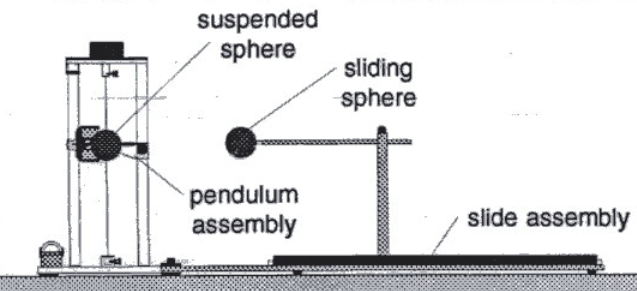
\includegraphics[width=0.8\textwidth]{Immagini/App.png}
    \caption{Apparato sperimentale: bilancia di torsione.} 
    \label{fig:Apparato}
\end{figure}

Come mostrato in Figura 1, una sfera leggera, ricoperta di vernice conduttiva, è sostenuta da un braccio rigidamente collegato ad un equipaggio mobile, contrappesato, ancorato a sua volta ad un sottile filo di torsione. La sfera può ruotare torcendo il filo. Una sfera identica è montata su un supporto a slitta, in modo che si possa posizionare a diverse distanze rispetto la prima. Per eseguire gli esperimenti, si caricano entrambe le sfere con carica dello stesso segno: la forza elettrostatica fra le due sfere causa l’allontanamento di quella mobile che, essendo vincolata al filo, si allontana ruotando di un certo angolo.
\newpage

\section{Dipendenza di \boldmath $F_C$ dalla distanza}
Si vuole verificare la dipendenza della forza di Coulomb dall’inverso del quadrato della distanza tra le cariche e, dal momento che nella bilancia di torsione l’angolo di torsione risulta direttamente proporzionale alla forza applicata, si può studiare la dipendenza dell’angolo di torsione $\theta$ dalla distanza r tra i centri delle sfere.

Si allontanano le due sfere alla massima distanza possibile, assumendo per ciascuna un diametro d = $(3.9 \pm 0.1)$ cm, e caricare entrambe ad un potenziale di 6 kV tramite una sonda di carica. Si procede portando la sfera mobile alla prima distanza selezionata: la forza repulsiva agente fra le due sfere farà ruotare l’equipaggio mobile appeso al filo di torsione. Si prosegua ruotando la manopola di azzeramento della torsione del filo fino a far coincidere lo zero dell’equipaggio mobile con quello fisso. Leggere il valore dell’angolo e ripetere il procedimento per diversi valori di r. I risultati delle misure sono riportati in Tabella 1. \\

\begin{table}[H]
\centering
\begin{tabular}{l l *{5}{S[table-format=3.2, table-number-alignment=center]}} 
\toprule
& & {\textbf{10cm}} & {\textbf{12cm}} & {\textbf{14cm}} & {\textbf{19cm}} & {\textbf{22cm}} \\
\midrule
& & 97.0 & 70.0 & 49.0 & 28.0 & 20.0 \\
& & 101.0 & 68.0 & 51.0 & 28.0 & 18.0 \\
& & 99.0 & 71.0 & 53.0 & 31.0 & 22.0 \\
\midrule
{\textbf{\boldmath$\bar{\theta}$}}         & {(\text{°})}    & 99.0 & 69.7 & 51.0 & 29.0 & 10.0 \\
{\textbf{\boldmath$\sigma_{\theta}$}}      & {(\text{°})}    & 2.0  & 1.5 & 2.0 & 1.7 & 2.0 \\
{\textbf{\boldmath$\bar{\sigma}_{\theta}$}} & {(\text{°})}    & 1.2  & 0.9 & 1.2 & 1.0 & 1.2 \\
\midrule
{\textbf{\boldmath$\bar{\theta}$}}         & {(\text{rad})}    & 1.73 & 1.22 & 0.89 & 0.51 & 0.35 \\
{\textbf{\boldmath$\sigma_{\theta}$}}      & {(\text{rad})}    & 0.03  & 0.03 & 0.03 & 0.03 & 0.03 \\
{\textbf{\boldmath$\bar{\sigma}_{\theta}$}} & {(\text{rad})}    & 0.02  & 0.02 & 0.02 & 0.02 & 0.02 \\
\bottomrule
\end{tabular}
\caption{Angoli di torsione e loro incertezza, errore standard della media in funzione della distanza r tra i centri delle sfere.}
\label{tab:distanza}
\end{table}

Le cariche sono libere di muoversi sulla superficie della sfera e, in assenza di forze elettrostatiche esterne, la loro distribuzione è uniforme sull'intera superficie: in queste condizioni, la sfera conduttrice carica si può approssimare ad una carica puntiforme posta nel centro della sfera. Tuttavia, quando le due sfere cariche sono vicine, le cariche mobili si
ridistribuiscono in modo da rendre minima l’energia elettrostatica, posizionandosi il più lontano possibile da quelle della sfera opposta. 
La distanza reale tra le cariche è quindi maggiore di quella tra i centri delle sfere, dunque la forza di Coulomb resulta minore. Questo effetto è particolarmente significativo quando la distanza tra le sfere è confrontabile con il loro raggio e dunque per tali valori la dipendenza lineare non è ben verificata.
\newpage
Correggere la relazione tra l’angolo $\theta$ e la distanza moltiplicando il valore dell’angolo per un fattore 1/B, con:

\begin{equation}
    B(r)=1-\frac{4a^3}{r^3}
    \label{1}
\end{equation}

dove $a$ è il raggio delle sfere.
Interpolare quindi i valori di $\theta$ corretti in funzione di $1/r^2$ determinando la miglior retta che descrive la relazione, come mostrato in Figura 2.

\begin{figure}[H]
    \centering
    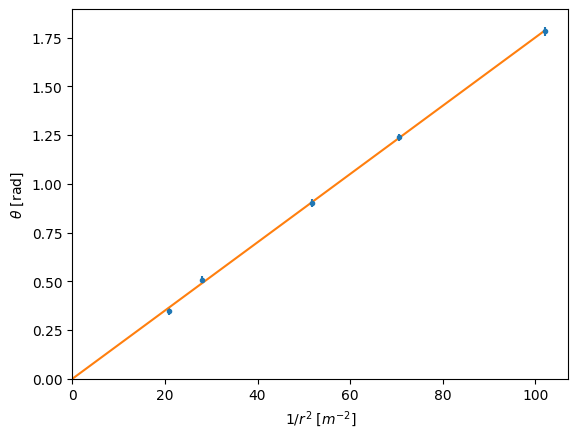
\includegraphics[width=0.8\textwidth]{Immagini/Distanza.png}
    \caption{Interpolazione lineare di $\theta$ corretto in funzione di $1/r^2$, usando un parametro e imponendo il passaggio per l'origine.} 
    \label{fig:Distanza}
\end{figure}

Il coefficiente angolare della retta interpolata è $k_1=(17.5 \pm 0.1) \cdot10^{-3}\: \text{m}^{2}$. Il test del $\chi^2$ della retta è $\tilde{\chi_o}^2= 0.44$, che per 4 gradi di libertà fornisce una probabilità di accordo con i dati del $78\%$.

\section{Dipendenza di \boldmath $F_C$ dalla carica}
\subsection{Potenziale Uguale}
Per determinare la dipendenza della forza di Coulomb dalla carica è necessario eseguire misure in modo analogo a quelle precedenti, mantenendo però fissa la distanza tra le due sfere: le misure sono state effettuate assumendo una distanza di $\qty{12.0 \pm 0.1}{cm}$. 
A piccole distanze la capacità delle sfere è circa costante, ed essendo la carica direttamente proporzionale al potenziale è sufficiente studiare la dipendenza della forza dal potenziale.
Caricare, dunque, le sfere allo stesso potenziale, in valori crescenti fino a 6 kV. Le misure sono state raccolte in tabella 2.

\begin{table}[H]
\centering
\begin{tabular}{S[table-format=4.0] S[table-format=2.0] S[table-format=2.0] S[table-format=1.2] S[table-format=1.2]} 
\toprule
{\textbf{Potenziale}} & {\textbf{$\sigma_V$}} & {\textbf{$\theta$}} & {\textbf{$\theta$}} & {\textbf{$\sigma_\theta$}} \\
{\text{(V)}}  & {\text{(V)}}  & {\text{(°)}} & {\text{(rad)}} & {\text{(rad)}} \\
\midrule
2000 & 10 & 10 & 0.17 & 0.07 \\
2500 & 10 & 14 & 0.24 & 0.07 \\
3000 & 10 & 20 & 0.35 & 0.07 \\
3500 & 10 & 23 & 0.40 & 0.07 \\
4000 & 10 & 35 & 0.61 & 0.07 \\
4500 & 10 & 41 & 0.72 & 0.07 \\
5000 & 10 & 48 & 0.84 & 0.07 \\
5500 & 10 & 62 & 1.08 & 0.07 \\
6000 & 10 & 70 & 1.22 & 0.07 \\
\bottomrule
\end{tabular}
\caption{Potenziale, angoli di torsione e relativa incertezza.}
\label{tab:potenziale_uguale}
\end{table}

Si interpolino linearmente gli angoli di torsione in funzione del potenziale $V^2$, applicando agli angoli la correzione 1/B, come in Figura 3.

\begin{figure}[H]
    \centering
    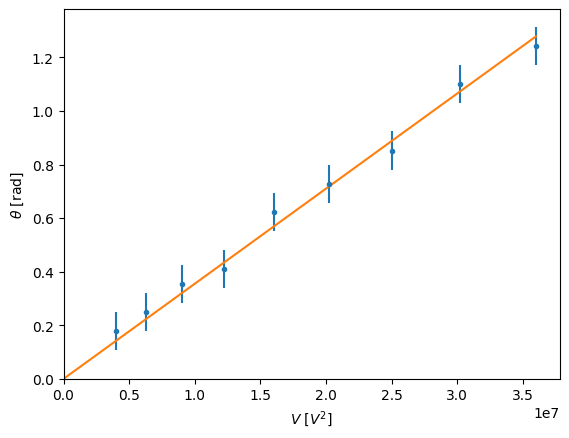
\includegraphics[width=0.8\textwidth]{Immagini/PotUguale.png}
    \caption{Interpolazione lineare di $\theta$ corretto in funzione di $V^2$, usando un parametro e imponendo il passaggio per l'origine.} 
    \label{fig:PotUguale}
\end{figure}

Il coefficiente angolare della retta interpolata è $k_2=(35 \pm 1)\: \text{nV}^{2}$. Il $\chi^2$ della retta è $\tilde{\chi_o}^2= 0.25$, che per 8 gradi di libertà fornisce una probabilità di accordo con i dati $98\%$.

\subsection{Potenziale Diverso}
Ripetere le misure mantenendo costante il potenziale su una sfera, valore assunto di 6kV, variandolo solo sull’altra. In Tabella 3 sono riportati i valori misurati.

\begin{table}[H]
\centering
\begin{tabular}{S[table-format=4.0] S[table-format=2.0] S[table-format=2.0] S[table-format=1.2] S[table-format=1.2]} 
\toprule
{\textbf{Potenziale}} & {\textbf{$\sigma_V$}} & {\textbf{$\theta$}} & {\textbf{$\theta$}} & {\textbf{$\sigma_\theta$}} \\
{\text{(V)}}  & {\text{(V)}}  & {\text{(°)}} & {\text{(rad)}} & {\text{(rad)}} \\
\midrule
6000 & 10 & 70 & 1.22 & 0.07 \\
5500 & 10 & 65 & 1.13 & 0.07 \\
5000 & 10 & 61 & 1.06 & 0.07 \\
4500 & 10 & 59 & 1.03 & 0.07 \\
4000 & 10 & 52 & 0.91 & 0.07 \\
3500 & 10 & 43 & 0.75 & 0.07 \\
3000 & 10 & 39 & 0.68 & 0.07 \\
2500 & 10 & 35 & 0.61 & 0.07 \\
2000 & 10 & 28 & 0.49 & 0.07 \\
\bottomrule
\end{tabular}
\caption{Potenziale, angoli di torsione e relative incertezze.}
\label{tab:potenziali_diversi}
\end{table}

Procedere con l'interpolazione lineare degli angoli di torsione in funzione del potenziale variabile, come mostrato in Figura 4.

\begin{figure}[H]
    \centering
    
\includegraphics[width=0.8\textwidth]{Immagini/PotDiverso.png}
    \caption{Interpolazione lineare di $\theta$ corretto in funzione di $V$, usando un parametro e imponendo il passaggio per l'origine.} 
    \label{fig:PotDiverso}
\end{figure}

La retta ha coefficiente angolare $k_3=(220 \pm 6) \mu \text{V}$. Il $\chi^2$ della retta è $\tilde{\chi_o}^2= 0.59$,che per 8 gradi di libertà fornisce una probabilità di accordo con i dati del $78\%$.

\section{Misura della costante di torsione del filo}
Per determinare la costante $C_{\text{tor}}/b$ si deve calibrare la bilancia di torsione utilizzando una forza nota che agisca sulla sfera mobile al posto della forza di Coulomb: si utilizza la forza di gravità. Collocare la bilancia sul fianco e posizionare un tubo di supporto sotto la sfera, per sostenerla fino a regolazione ultimata ed evitare torsioni eccessive del filo.
Azzerare la bilancia, ruotando la manopola di regolazione della torsione, fino a portare
l’indice inciso sul contrappeso a paletta in corrispondenza di quello inciso sul braccio
fisso: all’equilibrio, la bacchetta di sostegno della sfera mobile deve risultare perfettamente orizzontale.\\
Appoggiare cautamente una massa da 20 mg sulla sfera mobile e regolare la manopola della torsione fino a riportare la sfera nella posizione di equilibrio di partenza. Leggere, dunque, il valore dell’angolo di torsione e ripetere l'operazione con masse di valore crescente. 
Le misure sono riportate in Tabella 4.

\begin{table}[H]
\centering
\begin{tabular}{S[table-format=2.0] S[table-format=3.0] S[table-format=1.2] S[table-format=1.2]} 
\toprule
{\textbf{m (mg)}} & {\textbf{$\theta$ (°)}} & {\textbf{$\theta$ (rad)}} & {\textbf{$\sigma_\theta$ (rad)}} \\
\midrule
20 & 136 &  2.37 & 0.07 \\
40 & 282 &  4.92 & 0.07 \\
50 & 355 &  6.20 & 0.07 \\
70 & 500 &  8.73 & 0.07 \\
90 & 645 & 11.26 & 0.07 \\
\bottomrule
\end{tabular}
\caption{Massa, angoli di torsione e relative incertezze.}
\label{tab:costante:torsione}
\end{table}

All’equilibrio si possono eguagliare i momenti della forza di gravità $F_G$ e di quella torsione, e si ha $F_G \cdot b = m\cdot g \cdot b = C_{\text{tor}} \cdot \theta$,
dove b è il braccio della forza e $C_{\text{tor}}$ la costante di torsione del filo.
Una volta definito  $K_{\text{tor}} = C_{\text{tor}}/b$, si ottiene $m\cdot g = K_{\text{tor}}\cdot \theta$: interpolare linearmente i valori delle masse in funzione degli angoli di torsione, come in Figura 5.

\begin{figure}[H]
    \centering
    
\includegraphics[width=0.8\textwidth]{Immagini/Torsione.png}
    \caption{Interpolazione lineare di $\theta$ in funzione di $m$, usando un parametro e imponendo il passaggio per l'origine.} 
    \label{fig:Torsione}
\end{figure}

Dividendo $g$ per il coefficiente angolare interpolato si ottiene $K_{\text{tor}} = (78.8 \pm 0.3) \mu\text{N}$. Il test del $\chi^2$ per tale retta è $\tilde{\chi_o}^2= 1.06$, che per 4 gradi di libertà indica una probabilità di accordo con i dati del  $38\%$.

\section{Misura della costante dielettrica del vuoto}
Noto il valore di $K_{\text{tor}}$, si può quindi calcolare il valore della forza di Coulomb
corrispondente a ciascun valore di $\theta$ misurato precedentemente: infatti $F_C = K_{\text{tor}}\cdot \theta$.
Dalla relazione:

\begin{equation}
    F_C = \frac{4\pi \varepsilon_0 a^2V_1V_2}{r^2}
\end{equation}

è possibile ricavare la costante dielettrica del vuoto
$\varepsilon_0$, avendo approssimato $\varepsilon_r=1$ la costante
dielettrica relativa dell’aria.
A partire dai coefficienti angolari precedentemente interpolati, calcolare i valori di $\varepsilon_0$ e farne una media pesata: $\bar{\varepsilon_0} = (8.35 \pm 0.51)\cdot10^{-12}\text{C}^2/\text{Nm}^2$.

\section{Conclusioni}
L'esperienza ha permesso di effettuare tre misure indipendenti della costante dielettrica del vuoto tramite la legge di Coulomb e a quella del momento di torsione.
La media pesata $\bar{\varepsilon_0}$ delle tre misure risulta compatibile col valore previsto $\varepsilon_0 = 8.85\cdot10^{-12}\text{C}^2/\text{Nm}^2$ con una probabilità del $33\%$, corrispondente al valore calcolato di

\begin{equation}
    t_0=\frac{\abs{\varepsilon_0-\bar{\varepsilon_0}}}{\sigma_{\bar{\varepsilon_0}}}=0.97
\end{equation}

e, infatti, il valore di $\varepsilon_0$ è entro 1 $\sigma$ da quello misurato.

\section*{Riferimenti bibliografici}
\addcontentsline{toc}{section}{Riferimenti bibliografici}

\begin{enumerate}
    \raggedright
    \item[{[1]}] Marta Calvi. \textit{BILANCIA ELETTROSTATICA DI COULOMB}. Laboratorio I, Corso di Laurea in Fisica, A.A. 2025/26.
\end{enumerate}